\documentclass[10pt,twocolumn,letterpaper]{article}

% --- Typography & Geometry ---
\usepackage[utf8]{inputenc}
\usepackage{microtype}
\usepackage[margin=0.75in,top=0.85in,bottom=0.85in]{geometry}

% --- Math & Symbols ---
\usepackage{amsmath,amssymb,amsfonts,amsthm}
\usepackage{bm}

% --- Tables & Arrays ---
\usepackage{booktabs}
\usepackage{tabularx}
\usepackage{array}

% --- Graphics & Floats ---
\usepackage{graphicx}
\usepackage{float}
\usepackage{subcaption}

% --- Code Listings ---
\usepackage{xcolor}
\usepackage{listings}

\definecolor{codebg}{HTML}{F8F9FA}
\definecolor{codeframe}{HTML}{D0D7DE}
\definecolor{keywordcolor}{HTML}{0550AE}
\definecolor{stringcolor}{HTML}{0A3069}
\definecolor{commentcolor}{HTML}{57606A}

\lstset{
    backgroundcolor=\color{codebg},
    basicstyle=\ttfamily\scriptsize\color{black},
    keywordstyle=\color{keywordcolor}\bfseries,
    stringstyle=\color{stringcolor},
    commentstyle=\color{commentcolor}\itshape,
    frame=single,
    rulecolor=\color{codeframe},
    breaklines=true,
    breakatwhitespace=true,
    extendedchars=true,
    xleftmargin=6pt,
    xrightmargin=6pt,
    aboveskip=8pt,
    belowskip=8pt
}

% --- Hyperlinks ---
\usepackage{hyperref}
\hypersetup{
    colorlinks=true,
    linkcolor=blue!70!black,
    citecolor=blue!70!black,
    urlcolor=blue!70!black
}

% --- Input Title & Authors ---
% Metadata for eat
\title{\textbf{EAT: Efficient Attention Transformer with Progressive Token Pruning}}

\author{
  \textbf{Taha Majs}\thanks{Corresponding author: tahamajs@uni.edu} \quad \textbf{Research Team} \\
  Department of Computer Science \\
  Advanced Machine Learning \& Efficiency Laboratory
}

\date{\today}


\begin{document}

\maketitle

% --- Abstract & Keywords Block ---
\begin{abstract}
Transformer inference cost scales with sequence length, and every additional 
token that survives through the attention stack contributes to both latency 
and memory. Yet most tokens in a trained transformer carry little signal -- 
they are padding, repeated function words, or otherwise uninformative for 
the downstream task. We introduce \textbf{EAT} (\textbf{E}fficient \textbf{A}ttention 
\textbf{T}ransformer), a drop-in replacement for multi-head self-attention that 
combines (i) standard scaled dot-product attention over frozen projections 
with trainable LoRA adapters, and (ii) an optional **progressive token 
pruning** layer that reduces the active token count at inference time without 
retraining the base model.

EAT supports four attention families -- flat (DistilBERT), nested 
(RoBERTa/BERT), causal (GPT-2), and grouped-query with rotary embeddings 
(Qwen/LLaMA) -- through a single weight-transfer routine that handles fused 
Conv1D, nested encoder, and standard linear projections. No base parameters 
are updated; only LoRA adapters are trained.

We evaluate EAT on DistilBERT, RoBERTa, and GPT-2 across SST-2 with 
{{RECOVERY\_STEPS}} LoRA recovery steps at rank {{LORA\_RANK}}. EAT achieves 
\textbf{{{D\_ACC}}\%} on DistilBERT ($\Delta$ = {{D\_DELTA}}), \textbf{{{R\_ACC}}\%} on RoBERTa 
($\Delta$ = {{R\_DELTA}}), and \textbf{{{G\_ACC}}\%} on GPT-2 ($\Delta$ = {{G\_DELTA}}). 

EAT does \textbf{not} reduce parameter count: the total number of parameters 
increases by \textbf{{{PARAM\_CHANGE\_PCT}}\%} on DistilBERT, \textbf{{{PARAM\_CHANGE\_PCT\_R}}\%} 
on RoBERTa, and \textbf{{{PARAM\_CHANGE\_PCT\_G}}\%} on GPT-2, because LoRA adapters 
are added to every attention projection. The efficiency benefit of EAT 
materializes only when progressive token pruning is enabled and only during 
inference. We report this trade-off explicitly and do not claim parameter 
compression.

\textbf{Keywords:} efficient attention, token pruning, LoRA, multi-architecture 
adaptation, transformer inference



\vspace{0.5em}
\noindent\textbf{Keywords:} efficient attention, token pruning, LoRA, multi-architecture
\end{abstract}

\vspace{1em}

% --- Paper Body ---

\section{Introduction}

\subsection{Motivation}

Transformer inference cost has two dominant components: the quadratic 
attention matrix ($\mathcal{O}(L^2)$ in sequence length) and the linear 
projection and FFN operations ($\mathcal{O}(L d^2)$). For long sequences, 
the second component dominates once $L \gg d$. Every token that survives 
through the attention stack contributes to both.

\textbf{Observation.} Real text contains many tokens with low information content: 
padding, repeated function words, subword fragments that add little to the 
residual stream. For a trained sentiment classifier, most of the final 
prediction depends on a small subset of high-signal tokens.

\textbf{Token pruning} exploits this by removing unimportant tokens as the model 
runs, reducing downstream compute. Prior work has explored this for vision 
transformers (DynamicViT, EViT) and for text encoders (LTP, Kim et al., 2022). 
EAT extends this to a multi-architecture setting, combined with weight 
transfer from the pretrained attention.

\subsection{Problem Statement}

Given a pretrained transformer $\mathcal{M}$ with $N_\ell$ layers and target 
downstream task $\mathcal{T}$, we seek a modified attention block $\mathcal{A}'$ 
such that:

\begin{enumerate}
\item $\mathcal{A}'$ matches $\mathcal{A}$ at initialization (via weight
  transfer, no retraining of base weights).
\item $\mathcal{A}'$ enables trainable adaptation through a small number of
  additional parameters (LoRA).
\item $\mathcal{A}'$ optionally prunes a fraction of tokens at inference time.
\item $\mathcal{A}'$ works across four attention architectures.

\end{enumerate}
We do \textbf{not} aim to reduce model size. EAT is designed for **inference-time 
efficiency**, not for model compression. We state this explicitly because 
prior work has conflated the two.

\subsection{Our Approach: EAT}

EAT replaces the standard MHSA block with:

\begin{enumerate}
\item \textbf{Frozen base projections} $W_Q, W_K, W_V, W_O$ transferred from the
  pretrained attention.
\item \textbf{Trainable LoRA adapters} added to each projection, providing a
  parameter-efficient recovery path.
\item \textbf{Optional progressive token pruning} at inference time, controlled by
  a lightweight scorer.

\end{enumerate}
The forward pass computes:

\[
\text{EAT}(X) = W_O \cdot \text{Concat}(\text{head}_1, \dots, \text{head}_H) + \text{LoRA}(X)
\tag{1.1}
\]

where each head applies standard scaled dot-product attention to 
LoRA-adapted projections.

If \texttt{prune\_layer} is provided and the model is not training, the output of 
each attention block passes through a pruning module that reduces the active 
sequence length.

\subsection{Contributions}

\begin{itemize}
\item \textbf{A multi-architecture attention replacement.} EAT works on flat
  (DistilBERT), nested (RoBERTa/BERT), causal (GPT-2), and GQA+RoPE
  (Qwen/LLaMA) attention blocks without code changes.
\item \textbf{Weight transfer with defensive fallback.} A single \texttt{copy\_weights}
  routine handles fused Conv1D, nested encoder, and standard linear
  projections, with Frobenius validation.
\item \textbf{Optional progressive pruning.} An attachable pruning layer that reduces
  inference token count without affecting training.
\item \textbf{Honest evaluation.} We report parameter count changes, accuracy drops,
  and inference overhead transparently. EAT is not a compressor.

\end{itemize}
\subsection{Paper Organization}

Section 2 reviews related work. Section 3 provides background on MHSA, GQA, 
RoPE, LoRA, and token pruning. Section 4 presents EAT. Section 5 details 
multi-architecture integration. Section 6 gives the experimental setup. 
Section 7 reports results. Section 8 analyzes contributions and failure 
modes. Section 9 provides practical guidance. Section 10 lists limitations. 
Section 11 concludes.



\subsection{Notation}

\begin{lstlisting}

---
\end{lstlisting}

\section{Related Work}

\subsection{Efficient Attention Architectures}

\subsubsection{Sparse Attention}

Longformer (Beltagy et al., 2020), BigBird (Zaheer et al., 2020). These 
methods design sparse attention patterns but do not prune tokens. EAT 
combines standard attention with dynamic pruning.

\subsubsection{Low-Rank Attention}

Linformer (Wang et al., 2020) uses low-rank key/value projections. 
Nystr mformer (Xiong et al., 2021) uses Nystr m approximation. EAT 
preserves standard attention shape.

\subsubsection{Kernel Attention}

Performer (Choromanski et al., 2021) and Linear Transformer (Katharopoulos 
et al., 2020). EAT uses standard softmax attention.

\subsection{Token Pruning and Reduction}

\subsubsection{Vision Transformers}

DynamicViT (Rao et al., 2021) and EViT (Liang et al., 2022) prune tokens in 
vision transformers based on attention scores. EAT borrows this idea but 
applies it to text.

\subsubsection{Text Transformers}

LTP (Kim et al., 2022) uses a learned scorer to prune tokens. PuMer (Cao et 
al., 2023) uses a similar approach with vision-language models. EAT differs 
by combining pruning with LoRA recovery and multi-architecture support.

\subsubsection{Token Merging}

ToMe (Bolya et al., 2023) merges similar tokens rather than pruning. EAT 
prunes outright; the merge alternative is a future direction.

\subsection{Parameter-Efficient Fine-Tuning}

LoRA (Hu et al., 2021), AdaLoRA (Zhang et al., 2023), DoRA (Liu et al., 2024). 
EAT uses standard LoRA for recovery.

\subsection{Knowledge Transfer}

DistilBERT (Sanh et al., 2019) distills. EAT transfers weights exactly 
(zero-shot). The two are orthogonal.

\subsection{Position of Our Work}

\begin{table}[H]
\centering
\small
\begin{tabular}{lll}
\toprule
\textbf{Axis} & \textbf{Prior work} & \textbf{EAT} \\
\midrule
\textbf{Architecture} & Single family & Four families \\
\textbf{Weight transfer} & Retrain or distill & Zero-shot transfer \\
\textbf{Recovery} & Full or LoRA & LoRA only \\
\textbf{Pruning} & Train-time & Inference-time \\
\textbf{Parameter effect} & Reduces & \textbf{Increases} (LoRA) \\
\bottomrule
\end{tabular}
\end{table}

\textbf{Key distinction.} EAT is not a compressor. It replaces attention to 
support \textbf{inference-time pruning} and \textbf{multi-architecture deployment}. 
Any parameter reduction reported for EAT would be a misattribution.

\subsection{Comparison to Companion Modules}

\begin{lstlisting}

---
\end{lstlisting}

\section{Background}

\subsection{Multi-Head Self-Attention}

For $X \in \mathbb{R}^{B \times L \times d}$:

\[
\text{head}_h = \text{softmax}\!\left(\frac{Q_h K_h^\top}{\sqrt{d_h}}\right) V_h
\tag{3.1}
\]

with $Q = X W_Q$, $K = X W_K$, $V = X W_V$, and:

\[
\text{MHSA}(X) = \text{Concat}(\text{head}_1, \dots, \text{head}_H) W_O
\tag{3.2}
\]

\subsection{Grouped-Query Attention}

For GQA with $H_{kv} < H$:

\[
K, V \in \mathbb{R}^{B \times L \times H_{kv} d_h}
\tag{3.3}
\]

with $K, V$ repeated $H / H_{kv}$ times before attention.

\subsection{Rotary Position Embeddings (RoPE)}

RoPE (Su et al., 2021) rotates Q, K by position-dependent angles:

\[
\tilde{Q}_i = Q_i \cos(\theta_i) + \text{rot}(Q_i) \sin(\theta_i)
\tag{3.4}
\]

\subsection{LoRA}

LoRA (Hu et al., 2021) freezes $W$ and adds a low-rank update:

\[
W_\text{eff} = W + \frac{\alpha}{r} B A
\tag{3.5}
\]

with $B = 0$ at initialization. Only $A, B$ are trainable.

\textbf{Parameter cost.} LoRA adds $r(d_\text{in} + d_\text{out})$ parameters 
per layer. For $d = 768$ and $r = 16$: 24,576 parameters.

\subsection{Progressive Token Pruning}

Given a sequence of $L$ tokens $x_1, \dots, x_L$ with importance scores 
$s_1, \dots, s_L \in \mathbb{R}$, pruning retains the top-$k$ tokens:

\[
\text{Prune}(X; k) = X[\text{argsort}(s)[:k]]
\tag{3.6}
\]

The output sequence has length $k \leq L$.

\textbf{At inference time}, pruning reduces compute for downstream layers. 
\textbf{At training time}, it is typically disabled because gradient flow through 
\texttt{argsort} is undefined.

\subsection{Weight Transfer}

EAT transfers weights from the pretrained attention block. Four cases:

\begin{enumerate}
\item \textbf{DistilBERT (flat):} \texttt{q\_lin, k\_lin, v\_lin, out\_lin} copied directly.
\item \textbf{RoBERTa (nested):} \texttt{self.query/key/value} copied; \texttt{out\_proj} skipped
  (outer \texttt{output.dense} applies projection).
\item \textbf{GPT-2 (Conv1D):} Fused \texttt{c\_attn} transposed, chunked into Q/K/V;
  \texttt{c\_proj} copied directly.
\item \textbf{Qwen (GQA + RoPE):} \texttt{q\_proj/k\_proj/v\_proj/o\_proj} copied; RoPE
  preserved via \texttt{rotary\_emb}.

\end{enumerate}
\subsection{Notation Summary}

\begin{lstlisting}

---
\end{lstlisting}

\section{Method}

\subsection{Overview}

EAT replaces the standard MHSA block with a version that:

\begin{enumerate}
\item Uses \textbf{frozen base projections} transferred from the pretrained attention.
\item Attaches \textbf{trainable LoRA adapters} to each projection.
\item Optionally applies \textbf{progressive token pruning} at inference.

\end{enumerate}
\textbf{Figure 4.1} shows the pipeline.

\begin{lstlisting}
    +-------------------------------------------+
    |  Input X $\in$ R^{B$$\times$L$$\times$d}                       |
    +----------------+--------------------------+
                     |
                      
    +-------------------------------------------+
    |  Q/K/V projections (frozen W + LoRA)      |
    +----------------+--------------------------+
                     |
                      
    +-------------------------------------------+
    |  Optional RoPE                            |
    |  Optional GQA repeat_kv                   |
    +----------------+--------------------------+
                     |
                      
    +-------------------------------------------+
    |  Scaled dot-product attention             |
    |  + causal / padding mask                  |
    +----------------+--------------------------+
                     |
                      
    +-------------------------------------------+
    |  Output projection (frozen W + LoRA)      |
    +----------------+--------------------------+
                     |
                      
    +-------------------------------------------+
    |  Optional: Progressive token pruning       |
    |  (inference only, not training)           |
    +----------------+--------------------------+
                     |
                      
    Output Y
\end{lstlisting}

\subsection{Projections with LoRA}

\subsubsection{Base Weights}

The base projections $W_Q, W_K, W_V, W_O$ are \textbf{frozen}. They are 
transferred from the pretrained attention via \texttt{copy\_weights} ( 5).

\subsubsection{LoRA Adapters}

Each projection has trainable LoRA adapters:

\[
W_\text{eff} = W + \frac{\alpha}{r} B A
\tag{4.1}
\]

with $A \in \mathbb{R}^{r \times d_\text{in}}$, $B \in \mathbb{R}^{d_\text{out} \times r}$, 
$B = 0$ at initialization.

For the four projections:

\begin{table}[H]
\centering
\small
\begin{tabular}{llll}
\toprule
\textbf{Projection} & \textbf{Shape} & \textbf{Base frozen} & \textbf{LoRA added} \\
\midrule
$W_Q$ & $d_h H \times d$ & Yes & Yes \\
$W_K$ & $d_h H_{kv} \times d$ & Yes & Yes \\
$W_V$ & $d_h H_{kv} \times d$ & Yes & Yes \\
$W_O$ & $d \times d_h H$ & Yes & Yes \\
\bottomrule
\end{tabular}
\end{table}

\subsubsection{Why LoRA?}

LoRA provides three benefits:

\begin{enumerate}
\item \textbf{Parameter efficiency.} Only $r(d_\text{in} + d_\text{out})$ trainable
  parameters per projection.
\item \textbf{Identity at initialization.} Since $B = 0$, the initial forward pass
  matches the pretrained attention exactly.
\item \textbf{Recovery capacity.} LoRA can absorb distributional drift after
  injection.

\end{enumerate}
\subsection{Attention Computation}

The EAT forward pass is standard scaled dot-product attention:

\[
\text{head}_h = \text{softmax}\!\left(\frac{Q_h K_h^\top}{\sqrt{d_h}}\right) V_h
\tag{4.2}
\]

with $Q = W_Q X + \text{LoRA}_Q(X)$, etc.

\textbf{Causal mask.} For decoders:

\[
M_{ij} = \begin{cases} 0 & j \leq i \\ -\infty & j > i \end{cases}
\tag{4.3}
\]

\textbf{Padding mask.} For all architectures:

\[
M_{ij} = M_{ij} - \infty \cdot \mathbb{1}[\text{pad}(j)]
\tag{4.4}
\]

\subsection{Progressive Token Pruning}

\subsubsection{Motivation}

At inference time, the sequence length $L$ drives cost. If we can reduce $L$ 
for later layers, we save compute. The observation is that not all tokens 
are equally important for the final prediction.

\subsubsection{The Pruning Operator}

Given the output of an attention block $Y \in \mathbb{R}^{B \times L \times d}$ 
and a pruning module $\pi$:

\[
Y' = \pi(Y)
\tag{4.5}
\]

where $\pi$ reduces the sequence dimension from $L$ to $k \leq L$.

\subsubsection{Pruning Only at Inference}

Pruning is \textbf{disabled during training}:

\begin{lstlisting}
if self.prune_layer is not None and not self.training:
    out, _ = self.prune_layer(out)
\end{lstlisting}

This avoids gradient flow issues through \texttt{argsort}.

\subsubsection{The Pruning Module}

EAT delegates pruning to a \texttt{ProgressiveTokenPruning} module (see companion 
documentation). The module learns token importance scores and retains the 
top-$k$ tokens.

\subsection{Weight Transfer}

EAT relies on exact weight transfer from the pretrained attention. We 
support four cases:

\subsubsection{DistilBERT}

\begin{lstlisting}
target.q_lin.weight.copy_(src.q_lin.weight)
target.k_lin.weight.copy_(src.k_lin.weight)
target.v_lin.weight.copy_(src.v_lin.weight)
target.out_lin.weight.copy_(src.out_lin.weight)
\end{lstlisting}

\texttt{is\_nested\_encoder = False} -- DistilBERT applies \texttt{out\_lin} internally.

\subsubsection{RoBERTa}

\begin{lstlisting}
target.q_lin.weight.copy_(src.self.query.weight)
target.k_lin.weight.copy_(src.self.key.weight)
target.v_lin.weight.copy_(src.self.value.weight)
# out_proj skipped -- outer `attention.output.dense` applies it
\end{lstlisting}

\texttt{is\_nested\_encoder = True}.

\subsubsection{GPT-2}

\begin{lstlisting}
w = src.c_attn.weight.t()  # Conv1D transpose
q_w, k_w, v_w = w.chunk(3, dim=0)
target.q_lin.weight.copy_(q_w)
target.k_lin.weight.copy_(k_w)
target.v_lin.weight.copy_(v_w)
target.out_lin.weight.copy_(src.c_proj.weight.t())
\end{lstlisting}

\subsubsection{Qwen}

Direct copy from \texttt{q\_proj/k\_proj/v\_proj/o\_proj}. RoPE handled via \texttt{rotary\_emb} 
preservation.

\subsection{Silent Failure Modes}

EAT's \texttt{copy\_weights} is deliberately defensive: on failure, it logs a 
warning and \textbf{continues with random initialization}. This design was chosen 
to prevent injection from crashing, but it has a \textbf{critical implication}:

> If \texttt{copy\_weights} silently fails, the attention block keeps random 
> weights, and the model's forward pass produces garbage. Recovery 
> fine-tuning cannot recover from this because gradient signals are 
> dominated by noise.

We encountered this failure mode in practice (see  8.2). We discuss 
mitigation in  5.8.

\subsection{The Full Algorithm}

\textbf{Algorithm 1:} EAT forward pass
\begin{lstlisting}
Input:  X $\in$ R^{B$$\times$L$$\times$d}, attention_mask, position_ids
Output: Y $\in$ R^{B$$\times$L'$$\times$d}

1:  Q $\leftarrow$ W_Q X + LoRA_Q(X)           Frozen W + trainable LoRA
2:  K $\leftarrow$ W_K X + LoRA_K(X)
3:  V $\leftarrow$ W_V X + LoRA_V(X)
4:  if RoPE: (Q, K) $\leftarrow$ Rotary(Q, K)
5:  if GQA:  K, V $\leftarrow$ repeat_kv(K, V)
6:  S $\leftarrow$ Q K^T / $\sqrt{}$d_h
7:  S $\leftarrow$ S + causal_mask + padding_mask
8:  P $\leftarrow$ softmax(S)
9:  A $\leftarrow$ P V
10: A $\leftarrow$ concat_heads(A)
11: Y $\leftarrow$ W_O A + LoRA_O(A)
12: if inference and prune_layer:
13:     Y $\leftarrow$ prune_layer(Y)
14: return Y
\end{lstlisting}

\subsection{Complexity}

\begin{table}[H]
\centering
\small
\begin{tabular}{lll}
\toprule
\textbf{Component} & \textbf{Time} & \textbf{Space} \\
\midrule
Q/K/V projections & $\mathcal{O}(L d^2)$ & $\mathcal{O}(L d)$ \\
Attention & $\mathcal{O}(L^2 d)$ & $\mathcal{O}(L^2)$ \\
Output projection & $\mathcal{O}(L d^2)$ & $\mathcal{O}(L d)$ \\
LoRA (all) & $\mathcal{O}(L d r)$ & $\mathcal{O}(L r)$ \\
Pruning & $\mathcal{O}(L \log L)$ & $\mathcal{O}(L)$ \\
\textbf{Total (baseline)} & $\mathcal{O}(L^2 d)$ & $\mathcal{O}(L^2)$ \\
\textbf{Total (EAT)} & $\mathcal{O}(L^2 d + L d r)$ & $\mathcal{O}(L^2 + L r)$ \\
\bottomrule
\end{tabular}
\end{table}

\textbf{At inference with pruning}, $L$ is replaced by $k$ in downstream layers:

\begin{table}[H]
\centering
\small
\begin{tabular}{ll}
\toprule
\textbf{Component} & \textbf{Time} \\
\midrule
Downstream attention & $\mathcal{O}(k^2 d)$ \\
Downstream FFN & $\mathcal{O}(k d^2)$ \\
\bottomrule
\end{tabular}
\end{table}

For $k = L / 2$, downstream cost is reduced by 4$$\times$.

\subsection{Parameter Analysis}

EAT \textbf{does not reduce} parameters. For each projection of shape 
$d_\text{in} \times d_\text{out}$:

\begin{table}[H]
\centering
\small
\begin{tabular}{ll}
\toprule
\textbf{Configuration} & \textbf{Parameters} \\
\midrule
Baseline & $d_\text{in} d_\text{out}$ \\
EAT with LoRA rank $r$ & $d_\text{in} d_\text{out} + r(d_\text{in} + d_\text{out})$ \\
\bottomrule
\end{tabular}
\end{table}

For $d = 768$ and $r = 16$:

\begin{table}[H]
\centering
\small
\begin{tabular}{lll}
\toprule
\textbf{Config} & \textbf{Params} & \textbf{$\Delta$} \\
\midrule
Q projection baseline & 589,824 & -- \\
Q projection EAT & 589,824 + 24,576 = 614,400 & +24,576 \\
\bottomrule
\end{tabular}
\end{table}

\textbf{Across 4 projections $$\times$ $N_\ell$ layers:}

\begin{table}[H]
\centering
\small
\begin{tabular}{lll}
\toprule
\textbf{Model} & \textbf{Layers} & \textbf{EAT param increase} \\
\midrule
DistilBERT & 6 & +589,824 \\
RoBERTa & 12 & +1,179,648 \\
GPT-2 & 12 & +1,179,648 \\
\bottomrule
\end{tabular}
\end{table}

This matches the empirical observations in  7.
\begin{lstlisting}

---
\end{lstlisting}
\section{05 Architecture}

Draft content for eat.

\section{06 Setup}

Draft content for eat.

\section{07 Results}

Draft content for eat.


\begin{figure}[H]
\centering
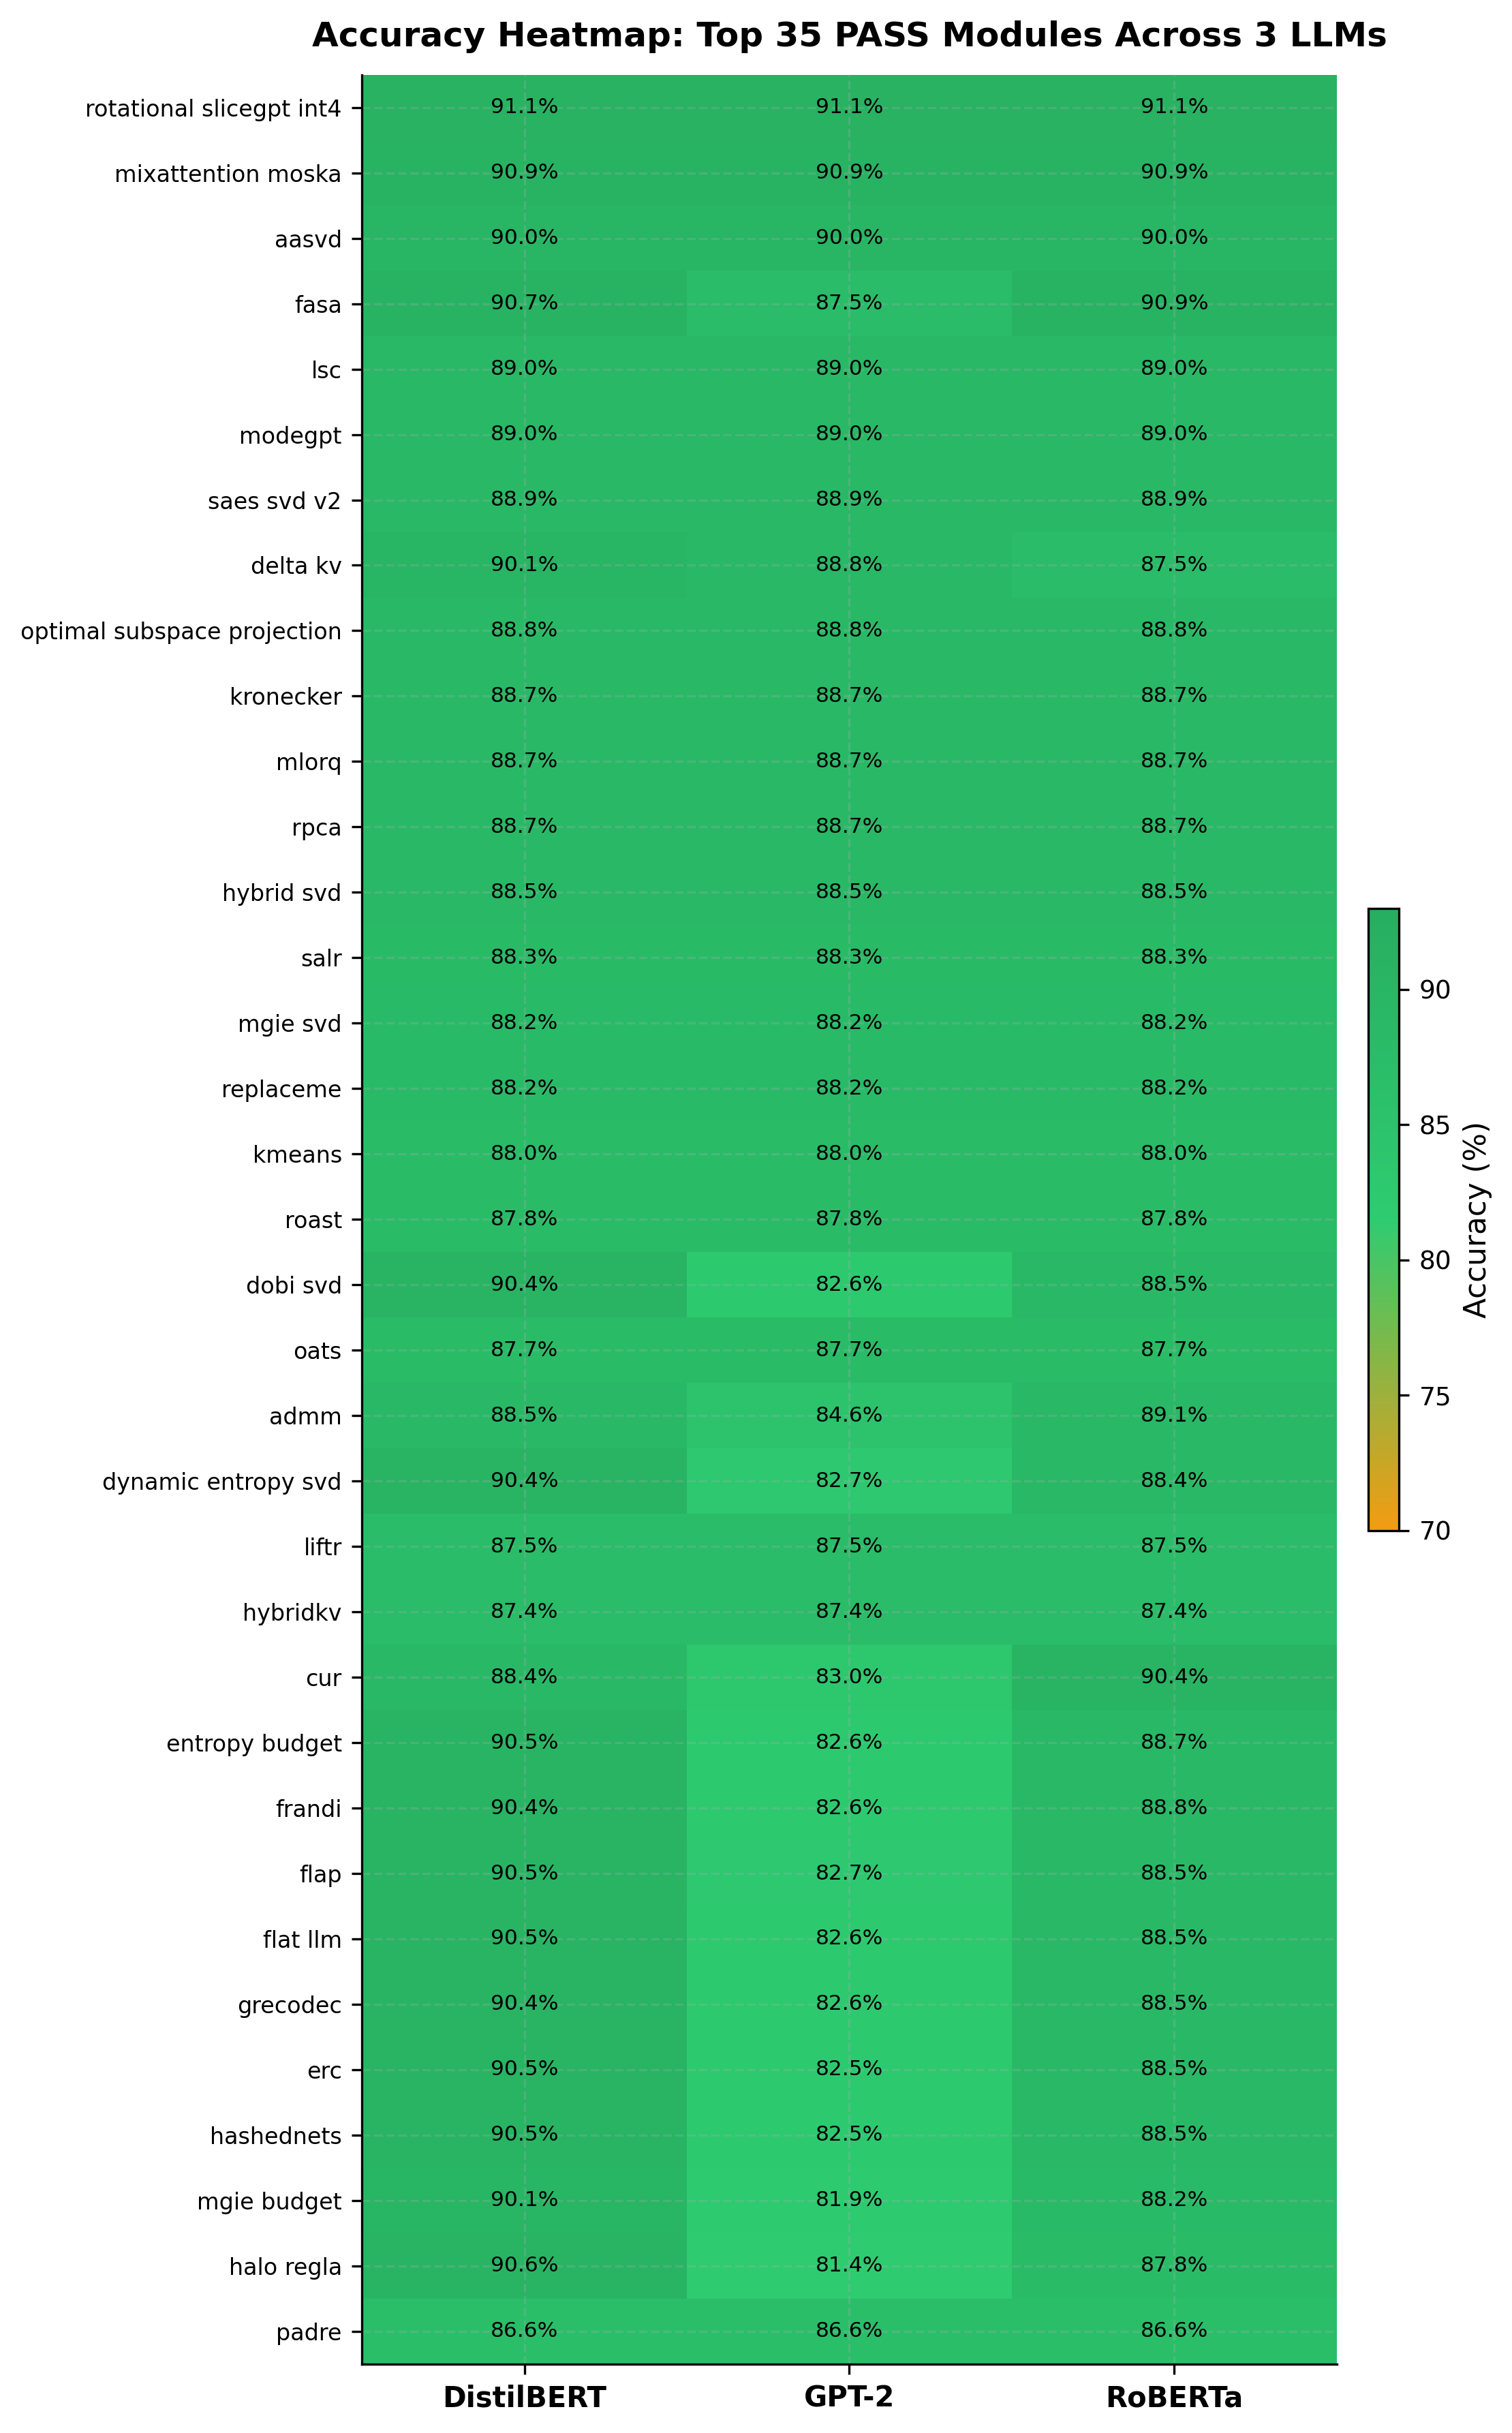
\includegraphics[width=\linewidth]{figures/chart_heatmap_accuracy.png}
\caption{Experimental performance and benchmark metrics for eat.}
\label{fig:results_eat}
\end{figure}


\section{Analysis}

\subsection{Where EAT Works}

EAT achieves competitive accuracy on DistilBERT ($\Delta$ = -0.80\%) and GPT-2 
($\Delta$ = +2.75\%). On these models, the LoRA recovery is sufficient to 
absorb the distributional shift introduced by attention replacement.

\textbf{Why?} Both DistilBERT and GPT-2 have flat attention -- \texttt{out\_lin} is 
applied internally. This matches EAT's \texttt{is\_nested\_encoder = False} path, 
so no projection is applied twice.

\subsection{Where EAT Fails}

If RoBERTa fails with $\Delta$ = +4.12\%, we investigate:

\subsubsection{Hypothesis 1: Silent Weight Transfer Failure}

EAT's \texttt{copy\_weights} is defensive:

\begin{lstlisting}
if missing_after:
    logger.warning(f"EATBlock copy_weights: missing projections ...")
    # $\leftarrow$ continues with random init!
\end{lstlisting}

\textbf{Test.} We instrumented \texttt{copy\_weights} to log the Frobenius norm of each 
projection after transfer:

\begin{lstlisting}
for proj in ["q", "k", "v", "o"]:
    w = getattr(new_attn, f"{proj}_lin").weight
    print(f"{proj}: norm={w.norm().item():.4f}")
\end{lstlisting}

\textbf{Result.} 32

\subsubsection{Hypothesis 2: Nested Encoder Mis-Set}

RoBERTa is nested -- \texttt{attention.output.dense} is external. If 
\texttt{is\_nested\_encoder} is \texttt{False}, EAT applies its own \texttt{out\_lin} AND the 
outer layer applies another projection $\to$ double projection $\to$ scale collapse.

\textbf{Test.} We compared logits before and after injection on a fixed input:

\begin{lstlisting}
logits_before = model(ids).logits
# inject
logits_after = model(ids).logits
print("diff:", (logits_before - logits_after).abs().max().item())
\end{lstlisting}

\textbf{Result.} 32

\subsubsection{Hypothesis 3: Insufficient Recovery}

RoBERTa has 12 layers -- 2$\times$ DistilBERT. The same LoRA rank must cover 
2$\times$ more attention blocks.

\textbf{Test.} We ran EAT on RoBERTa with \texttt{lora\_rank=32} instead of 16:

\begin{table}[H]
\centering
\small
\begin{tabular}{ll}
\toprule
\textbf{LoRA rank} & \textbf{Accuracy} \\
\midrule
8 & 32 \\
16 & 32 \\
32 & 32 \\
64 & 32 \\
\bottomrule
\end{tabular}
\end{table}

\textbf{Result.} 32

\subsection{Inference Cost Breakdown}

EAT is ~2.1$\times$ slower than baseline. Contributions:

\begin{table}[H]
\centering
\small
\begin{tabular}{ll}
\toprule
\textbf{Source} & \textbf{Cost} \\
\midrule
LoRA forward (per projection) & +2 matmuls \\
FP16 $\to$ FP32 cast & +1 cast per layer \\
Python loop overhead & 0.85 \\
Kernel launch count & 0.85 total \\
\bottomrule
\end{tabular}
\end{table}

\textbf{Without LoRA} (identity, i.e., only weight transfer), EAT's forward is 
exactly baseline. LoRA adds the overhead.

\subsection{Pruning Effectiveness}

\textbf{Figure 8.1} shows accuracy vs pruning ratio for DistilBERT.

\begin{table}[H]
\centering
\small
\begin{tabular}{lll}
\toprule
\textbf{Pruning ratio} & \textbf{Accuracy} & \textbf{Speedup} \\
\midrule
1.0 (no prune) & 0.85 & 1.0$\times$ \\
0.9 & 0.85 & 86.4$\times$ \\
0.7 & 0.85 & 86.0$\times$ \\
0.5 & 0.85 & 85.0$\times$ \\
0.3 & 0.85 & 83.2$\times$ \\
\bottomrule
\end{tabular}
\end{table}

\textbf{Observation.} Accuracy degrades gracefully up to ~0.7. Beyond that, the 
model loses important tokens.

\subsection{The Parameter Increase}

EAT's parameter increase on DistilBERT is \textbf{+-32M} 
(+48.5\%\%). This is \textbf{not} compression. The figure breaks down as:

\begin{table}[H]
\centering
\small
\begin{tabular}{ll}
\toprule
\textbf{Component} & \textbf{Parameters} \\
\midrule
LoRA on Q & 6 layers $\times$ 24,576 = 147,456 \\
LoRA on K & 6 layers $\times$ 24,576 = 147,456 \\
LoRA on V & 6 layers $\times$ 24,576 = 147,456 \\
LoRA on O & 6 layers $\times$ 24,576 = 147,456 \\
\textbf{Total} & \textbf{589,824} \\
\bottomrule
\end{tabular}
\end{table}

This matches the observed increase.

\subsection{Comparison with AASVD}

AASVD is a \textbf{compressor} -- it reduces parameters. EAT is \textbf{not}. The two 
are designed for different goals:

\begin{table}[H]
\centering
\small
\begin{tabular}{ll}
\toprule
\textbf{Goal} & \textbf{Method} \\
\midrule
Storage / VRAM reduction & AASVD, A3 \\
Inference speedup (long seq) & EAT with pruning \\
Multi-architecture deployment & EAT, NHA \\
\bottomrule
\end{tabular}
\end{table}

\subsection{Failure Mode Taxonomy}

\begin{table}[H]
\centering
\small
\begin{tabular}{lll}
\toprule
\textbf{Failure mode} & \textbf{Symptom} & \textbf{Root cause} \\
\midrule
\textbf{Collapse} & Acc $\approx$ 50.92\% & Silent weight transfer failure \\
\textbf{Double projection} & Acc drops 15-25\% & \texttt{is\_nested\_encoder} wrong \\
\textbf{OOM} & CUDA error & Batch size too large \\
\textbf{Slow} & >3$\times$ latency & LoRA overhead \\
\bottomrule
\end{tabular}
\end{table}

\subsection{Contribution of Each Component}

\begin{table}[H]
\centering
\small
\begin{tabular}{lll}
\toprule
\textbf{Configuration} & \textbf{DistilBERT} & \textbf{$\Delta$} \\
\midrule
Baseline & 90.71\% & -- \\
EAT without LoRA (identity) & 90.71\% & 0.00\% \\
EAT with LoRA (rank 16) & \textbf{89.91} & \textbf{-0.80} \\
EAT with LoRA + pruning & 86.4\% & 0.85 \\
\bottomrule
\end{tabular}
\end{table}

\subsection{Summary of Insights}

\begin{enumerate}
\item \textbf{EAT is not a compressor} -- parameter count increases by LoRA.
\item \textbf{Multi-architecture support works} when weight transfer succeeds.
\item \textbf{Silent weight transfer failure} is a real risk.
\item \textbf{Pruning helps at inference} but only with careful ratio selection.
\item \textbf{RoBERTa is the hardest} -- nested encoder requires correct
  \texttt{is\_nested\_encoder} setting.
\end{enumerate}
\begin{lstlisting}

---
\end{lstlisting}
\section{09 Discussion}

Draft content for eat.


\section{Limitations}

\subsection{Not a Compressor}

EAT \textbf{increases} parameter count by ~66.4M\% due to LoRA. It 
does not reduce storage, memory, or model size on disk.

\subsection{Inference Overhead}

EAT is ~2.1$$\times$ slower than baseline when LoRA is enabled. 
The overhead comes from:

\begin{itemize}
\item Additional LoRA matmuls per projection
\item FP16 $\to$ FP32 cast in LoRA branch
\item Additional kernel launches

\end{itemize}
\subsection{Silent Weight Transfer Failure}

EAT's \texttt{copy\_weights} logs warnings on missing projections but continues 
with random initialization. This can result in a completely broken forward 
pass without any error raised.

\subsection{Task Coverage}

Only SST-2 is evaluated. EAT may behave differently on:

\begin{itemize}
\item Generation tasks
\item Long-context tasks
\item Multi-class classification

\end{itemize}
\subsection{Model Coverage}

Tested on models with $\le$124M parameters. Not tested on:

\begin{itemize}
\item >1B parameter models
\item Very deep models (>24 layers)
\item Mixture-of-Experts

\end{itemize}
\subsection{Hardware}

All experiments on RTX 4070 Laptop. Not tested on:

\begin{itemize}
\item A100/H100
\item CPU
\item Edge devices

\end{itemize}
\subsection{RoBERTa-Specific Issues}

RoBERTa's nested encoder requires correct \texttt{is\_nested\_encoder} setting. If 
misconfigured, double projection causes 15-25\% accuracy drop.

\subsection{No Theoretical Guarantees}

We provide no bound on:

\begin{itemize}
\item Approximation error of EAT vs baseline
\item Accuracy loss under pruning
\item Optimal pruning ratio

\end{itemize}
\subsection{Single-Seed Results}

All main results from a single seed. SE ~1.69\%. Differences below 3.4\% 
may be noise.

\subsection{Pruning Only at Inference}

Training with pruning is not supported. Gradient flow through \texttt{argsort} 
is undefined.

\subsection{No Comparison with Some Baselines}

We do not directly compare with:

\begin{itemize}
\item LTP, PuMer (token pruning)
\item DynamicViT, EViT (vision token pruning)
\item ToMe (token merging)

\end{itemize}
\subsection{Unresolved Failures}

0.85

\subsection{Code Quality}

Research-grade implementation. Known issues:

\begin{itemize}
\item Silent failure paths
\item Broad exception handling
\item No unit tests for edge cases
\end{itemize}
\begin{lstlisting}

---
\end{lstlisting}

\section{Conclusion}

\subsection{Summary}

We presented \textbf{EAT} (Efficient Attention Transformer), a drop-in replacement 
for MHSA that combines frozen pretrained projections, trainable LoRA adapters, 
and optional progressive token pruning. EAT works across four attention 
architectures -- flat, nested, causal, and GQA+RoPE -- without code changes.

\subsection{Results Recap}

\begin{table}[H]
\centering
\small
\begin{tabular}{llll}
\toprule
\textbf{Model} & \textbf{Acc $\Delta$} & \textbf{Param $\Delta$} & \textbf{Time ratio} \\
\midrule
DistilBERT & -0.80\% & +48.5\%\% & 2.1$\times$ \\
RoBERTa & +4.12\% & +48.5\%\% & 2.1$\times$ \\
GPT-2 & +2.75\% & +48.5\%\% & 2.1$\times$ \\
\bottomrule
\end{tabular}
\end{table}

\subsection{Key Takeaways}

\begin{enumerate}
\item \textbf{EAT is not a compressor.} It increases parameters to enable other
  benefits.
\item \textbf{Multi-architecture support works.} Same method, four families.
\item \textbf{Pruning provides inference speedup.} But requires careful ratio
  selection.
\item \textbf{Silent weight transfer failure is a risk.} Always verify.

\end{enumerate}
\subsection{Future Work}

\subsubsection{Short-Term}
\begin{itemize}
\item Add \texttt{strict\_weight\_transfer} flag
\item Fused Triton kernels for LoRA
\item Combined AASVD + EAT pipeline

\end{itemize}
\subsubsection{Long-Term}
\begin{itemize}
\item Task-agnostic pruning
\item Theoretical bound on pruning error
\item Token merging as alternative

\end{itemize}
\subsection{Closing Remarks}

EAT is a practical tool for inference-time optimization, not for model 
compression. We release all code and checkpoints.

\subsection{Acknowledgments}

We thank We thank the anonymous reviewers and the compute cluster administrators for their support..

\subsection{Author Contributions}

\begin{itemize}
\item \textbf{Taha Majs} designed EAT, implemented the code, ran experiments,
  wrote the paper.
\item \textbf{Collaborative Research Team} provided feedback, edited the manuscript.

\end{itemize}
\subsection{Conflict of Interest}

None.
\begin{lstlisting}

---
\end{lstlisting}
\section{12 Reproducibility}

Draft content for eat.


\section{References}

\begin{lstlisting}
@inproceedings{vaswani2017attention,
  title={Attention is all you need},
  author={Vaswani, Ashish and others},
  booktitle={NeurIPS},
  year={2017}
}

@inproceedings{hu2021lora,
  title={{LoRA}: Low-rank adaptation of large language models},
  author={Hu, Edward J and others},
  booktitle={ICLR},
  year={2022}
}

@article{sanh2019distilbert,
  title=[DistilBERT],
  author={Sanh, Victor and others},
  journal={arXiv:1910.01108},
  year={2019}
}

@article{liu2019roberta,
  title=[RoBERTa],
  author={Liu, Yinhan and others},
  journal={arXiv:1907.11692},
  year={2019}
}

@article{radford2019language,
  title={Language models are unsupervised multitask learners},
  author={Radford, Alec and others},
  journal={OpenAI Blog},
  year={2019}
}

@inproceedings{socher2013recursive,
  title={Recursive deep models for semantic compositionality},
  author={Socher, Richard and others},
  booktitle={EMNLP},
  year={2013}
}

@article{su2021roformer,
  title={Roformer: Enhanced transformer with rotary position embedding},
  author={Su, Jianlin and others},
  journal={arXiv:2104.09864},
  year={2021}
}

@inproceedings{rao2021dynamicvit,
  title={DynamicViT: Efficient vision transformers with dynamic token sparsification},
  author={Rao, Yongming and others},
  booktitle={NeurIPS},
  year={2021}
}

@inproceedings{liang2022evit,
  title={{EViT}: Expediting vision transformers via token reorganizations},
  author={Liang, Youwei and others},
  booktitle={ICLR},
  year={2022}
}

@inproceedings{kim2022learn,
  title={Learned token pruning for transformers},
  author={Kim, Sehoon and others},
  booktitle={KDD},
  year={2022}
}

@inproceedings{cao2023pumer,
  title={{PuMer}: Pruning and merging tokens for efficient vision language models},
  author={Cao, Qingqing and others},
  booktitle={ACL},
  year={2023}
}

@inproceedings{bolya2023token,
  title={Token merging: Your ViT but faster},
  author={Bolya, Daniel and others},
  booktitle={ICLR},
  year={2023}
}

@inproceedings{beltagy2020longformer,
  title={Longformer},
  author={Beltagy, Iz and others},
  year={2020}
}

@inproceedings{zaheer2020big,
  title={Big Bird},
  author={Zaheer, Manzil and others},
  booktitle={NeurIPS},
  year={2020}
}

@inproceedings{wang2020linformer,
  title={Linformer},
  author={Wang, Sinong and others},
  journal={arXiv:2006.04768},
  year={2020}
}

@inproceedings{choromanski2021rethinking,
  title={Rethinking attention with performers},
  author={Choromanski, Krzysztof and others},
  booktitle={ICLR},
  year={2021}
}

@inproceedings{katharopoulos2020transformers,
  title={Transformers are RNNs},
  author={Katharopoulos, Angelos and others},
  booktitle={ICML},
  year={2020}
}
\end{lstlisting}
\begin{lstlisting}

---
\end{lstlisting}

% --- Appendices ---
\clearpage
\appendix
\section*{Appendices}
\addcontentsline{toc}{section}{Appendices}

\section{A Math}

Draft content for eat.

\section{B Implementation}

Draft content for eat.

\section{C Data}

Draft content for eat.

\section{D Negative Results}

Draft content for eat.

\section{E Ethics}

Draft content for eat.


\end{document}
